\documentclass[10pt,letterpaper]{article}

\usepackage[margin=1in]{geometry}
\usepackage{amsmath,amssymb}
\usepackage{graphicx}
\usepackage{float}
\usepackage{booktabs}
\usepackage{array}
\usepackage{parskip}
\usepackage{fancyhdr}
\usepackage{enumitem}
\usepackage{hyperref}
\usepackage{xcolor}
\usepackage{parskip}
\usepackage{minted, mdframed}
\usepackage{hyperref}
\hypersetup{
colorlinks=true,
linkcolor=blue, %purple
citecolor= blue,
urlcolor=cyan
}

\usepackage[utf8]{inputenc}
\usepackage{tikz}
% \usetikzlibrary{shapes.geometric, arrows.meta, calc, positioning}
\usetikzlibrary{arrows.meta, calc, positioning, shapes.gates.logic.US, shapes.geometric}


\pagestyle{fancy}
\fancyhf{}
\lhead{CS M151A: Introduction to Digital Design Lab}
\rhead{Lab 1 - Sequencer}
\cfoot{\thepage}

\newcommand{\unit}[1]{\text{ #1}}

\title{\textbf{Lab 1 - Sequencer}}
\author{Don D. Le and Gaurav Kumar}
\date{Spring 2026}

\begin{document}

\maketitle
\tableofcontents
\listoffigures
\addcontentsline{toc}{section}{\listfigurename}
\clearpage

% ============================================================

\section{Demonstration}


\begin{enumerate}
    \item \textbf{(Demo)} Build the project using based on the source files in \texttt{src.zip}, and make sure that it works. Translate the following ``program'' into binary instructions. Demo the UART console output to your TA after you finish.
    
    \begin{itemize}
        \item \texttt{PUSH R0 0x4}
        \item \texttt{PUSH R0 0x0}
        \item \texttt{PUSH R1 0x3}
        \item \texttt{MULT R0 R1 R2}
        \item \texttt{ADD R2 R0 R3}
        \item \texttt{MULT R1 R3 R3}
        \item \texttt{SEND R0}
        \item \texttt{SEND R1}
        \item \texttt{SEND R2}
        \item \texttt{SEND R3}
    \end{itemize}

    \textit{Answer.} Demo below, based on result from the actual board:

    \begin{figure}[H]
        \centering
        \includegraphics[width=0.75\linewidth]{image1.png}
        \caption{Putty Output}
        \label{fig:putty}
    \end{figure}
    
    \item \textbf{(Demo)} Read the testbench code and finish workshop 2. 

    \textit{Answer.} Completed in section 3
    
    \item \textbf{(Report)} Read the implementation code and finish workshop 1. Include answers in the report. Note that the lab report format described in the syllabus does not apply to this lab.

    \textit{Answer.} Completed in section 2
\end{enumerate}

\section{Workshop 1}
\subsection{Clock Dividers}

In the \texttt{basys3.v} file, there is a signal/reg named \texttt{clk\_en}. The \texttt{clk\_en} represents a clock that is much slower than the master clock \texttt{clk}. Read the section of code that’s relevant to \texttt{clk\_en} and try to understand how the clock divider is implemented.

\textit{Answer.} The clock divider is implemented in the code section below:\\

\begin{mdframed}
\begin{minted}[fontsize=\footnotesize]{verilog}
// ===========================================================================
// 763Hz timing signal for clock enable
// ===========================================================================

assign clk_dv_inc = clk_dv + 1;

always @ (posedge clk)
  if (rst)
    begin
       clk_dv   <= 0;
       clk_en   <= 1'b0;
       clk_en_d <= 1'b0;
    end
  else
    begin
       clk_dv   <= clk_dv_inc[16:0];
       clk_en   <= clk_dv_inc[17];
       clk_en_d <= clk_en;
    end
\end{minted}
\end{mdframed}

How it works: the input clock, \verb|clk| is 100 MHz, which is way too big and too fast for any meaningful interaction for humans, so we slow it down using \verb|clk_en|

\textbf{Questions.}
\begin{enumerate}
    \item Add \texttt{clk\_en} to the simulation’s waveform tab and then run the simulation again. Use the cursor to find the periodicity of this signal (you can select the signal and use arrow keys to reach the exact edges). Capture a waveform picture that shows two occurrences of \texttt{clk\_en}, and include it in the lab report. Indicate the exact period of the signal in the report.

    \textit{Answer.} Waveform picture is shown below

    \begin{figure}[H]
        \centering
        \includegraphics[width=0.9\linewidth]{gk_1.png}
        \caption{Two instances of \texttt{clk\_en}}
        \label{fig:gk1}
    \end{figure}

    We start tracking the simulation at 1,000.000 ns, and the end of the first edge was at 1,311,745.000 ns. Therefore the period is
    \[
    T = 1,311,745.000 - 1,000.000 = 1,310,745.000 \;\mathrm{ns} \approx 1310.75 \;\mu\text{s}
    \]
    However, the first period is not the correct answer. We found out that for the following periods, they slowly converge to the following value:
    \[
    6554.625 - 5243.905 = 1310.72\;\mu\text{s}
    \]
    
    \item A duty cycle is the percentage of one period in which a signal or system is active:
    \[
    D = \frac{T}{P} \times 100\%
    \]
    where $D$ is the duty cycle, $T$ is the interval where the signal is high, and $P$ is the period. What is the exact duty cycle of \texttt{clk\_en} signal?

    \textit{Answer.} The active time is simply the peak of the wave, which is 10 ns, so the duty cycle is
    \[
    D = \frac{T}{P}\times 100\% = \frac{10\unit{ns}}{1310.72\times 10^3\unit{ns}}\times 100\% = 0.00076\%
    \]
    
    \item What is the value of \texttt{clk\_dv} signal during the clock cycle that \texttt{clk\_en} is high?

    \textit{Answer.} \verb|clk_dv| is zero when \verb|clk_en| is high. See the picture below

    \begin{figure}[H]
        \centering
        \includegraphics[width=0.8\linewidth]{clk-dv.png}
        \caption{Instances of \texttt{clk\_dv} is zero when \texttt{clk\_en} is high}
        \label{fig:clk-dv}
    \end{figure}
    
    \item Draw a simple schematic/diagram of signals \texttt{clk\_dv}, \texttt{clk\_en}, and \texttt{clk\_en\_d} signals. It should be a translation of the corresponding Verilog code.

    \textit{Answer.} See the diagram below.

    \begin{figure}[H]
    \centering
    \resizebox{0.95\linewidth}{!}{%
    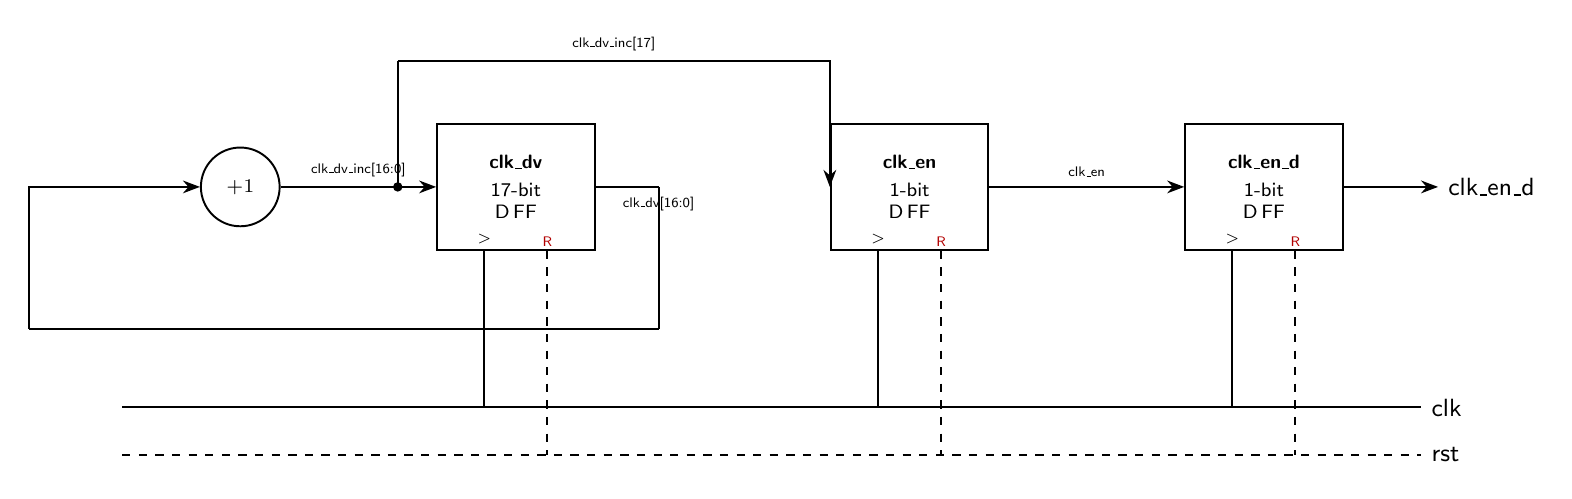
\begin{tikzpicture}[
        font=\sffamily\small,
        >=Stealth,
        line width=0.7pt,
        reg/.style={
            draw, rectangle,
            minimum width=2.0cm,
            minimum height=1.6cm,
            align=center,
            font=\sffamily\scriptsize
        },
        adder/.style={
            draw, circle,
            minimum size=1.0cm,
            align=center,
            font=\sffamily\scriptsize
        },
    ]

    %============================================================
    % 17-bit register: clk_dv
    %============================================================
    \node[reg] (REGDV) at (0,0) {{\bfseries clk\_dv}\\[2pt]17-bit\\D\,FF};

    % Port coordinates
    \coordinate (REGDV-D)   at (REGDV.west);
    \coordinate (REGDV-Q)   at (REGDV.east);
    \coordinate (REGDV-CLK) at ($(REGDV.south)+(-0.4,0)$);
    \coordinate (REGDV-RST) at ($(REGDV.south)+(0.4,0)$);

    %============================================================
    % Adder: clk_dv + 1 = clk_dv_inc
    %============================================================
    \node[adder] (ADD) at (-3.5, 0) {$+1$};

    % Feedback path: Q → adder → D
    \draw[->] (ADD.east) -- node[above, font=\sffamily\tiny] {clk\_dv\_inc[16:0]} (REGDV-D);

    % Feedback loop: clk_dv Q out → down → left → up → adder in
    \draw (REGDV-Q) -- ++(0.8,0) coordinate (fbr);
    \draw (fbr) -- ++(0,-1.8) coordinate (fbb);
    \draw (fbb) -- ++(-8.0,0) coordinate (fbl);
    \draw[->] (fbl) -- (fbl |- ADD.west) -- (ADD.west);
    \node[font=\sffamily\tiny, below] at (fbr) {clk\_dv[16:0]};

    %============================================================
    % D-FF: clk_en (latches clk_dv_inc[17])
    %============================================================
    \node[reg] (REGCE) at (5.0, 0) {{\bfseries clk\_en}\\[2pt]1-bit\\D\,FF};
    \coordinate (REGCE-D)   at (REGCE.west);
    \coordinate (REGCE-Q)   at (REGCE.east);
    \coordinate (REGCE-CLK) at ($(REGCE.south)+(-0.4,0)$);
    \coordinate (REGCE-RST) at ($(REGCE.south)+(0.4,0)$);

    % Wire: clk_dv_inc[17] → clk_en D
    % Tap from adder output, route up and over
    \coordinate (tap17) at (-1.5, 0);
    \fill (tap17) circle[radius=0.06];
    \draw (tap17) -- ++(0, 1.6) coordinate (tap17u);
    \draw[->] (tap17u) -- (tap17u -| REGCE-D) -- (REGCE-D);
    \node[font=\sffamily\tiny, above] at ($(tap17u)!0.5!(tap17u -| REGCE-D)$) {clk\_dv\_inc[17]};

    %============================================================
    % D-FF: clk_en_d (latches clk_en)
    %============================================================
    \node[reg] (REGCED) at (9.5, 0) {{\bfseries clk\_en\_d}\\[2pt]1-bit\\D\,FF};
    \coordinate (REGCED-D)   at (REGCED.west);
    \coordinate (REGCED-Q)   at (REGCED.east);
    \coordinate (REGCED-CLK) at ($(REGCED.south)+(-0.4,0)$);
    \coordinate (REGCED-RST) at ($(REGCED.south)+(0.4,0)$);

    % Wire: clk_en Q → clk_en_d D
    \draw[->] (REGCE-Q) -- node[above, font=\sffamily\tiny] {clk\_en} (REGCED-D);

    % Output
    \draw[->] (REGCED-Q) -- ++(1.2,0) node[right] {clk\_en\_d};

    %============================================================
    % CLK bus
    %============================================================
    \def\clky{-2.8}
    \draw (-5, \clky) -- (11.5, \clky) node[right] {clk};
    \foreach \ff in {REGDV, REGCE, REGCED}{
        \draw (\ff-CLK) -- (\ff-CLK |- 0,\clky);
        \node[font=\sffamily\tiny] at ($(\ff-CLK)+(0,0.15)$) {$\mathbf{>}$};
    }

    %============================================================
    % RST bus
    %============================================================
    \def\rsty{-3.4}
    \draw[dashed] (-5, \rsty) -- (11.5, \rsty) node[right] {rst};
    \foreach \ff in {REGDV, REGCE, REGCED}{
        \draw[dashed] (\ff-RST) -- (\ff-RST |- 0,\rsty);
        \node[font=\sffamily\tiny, text=red!70!black] at ($(\ff-RST)+(0,0.12)$) {R};
    }

    \end{tikzpicture}
    }
    \caption{Clock divider schematic: \texttt{clk\_dv}, \texttt{clk\_en}, and \texttt{clk\_en\_d}}
    \end{figure}

    The 17-bit register \texttt{clk\_dv} acts as a free-running counter incremented each clock cycle. When it overflows (bit~17 of \texttt{clk\_dv\_inc} goes high), \texttt{clk\_en} is asserted for one clock cycle. \texttt{clk\_en\_d} is simply a one-cycle delayed copy of \texttt{clk\_en}.

\end{enumerate}

\subsection{Debouncing}

Now move on to the signal \texttt{inst\_vld}. Read the relevant code and use the simulation as your aid, answer the following questions in your lab report.

\textbf{Questions.}
\begin{enumerate}
    \item What is the purpose of \texttt{clk\_en\_d} signal when used in expression \texttt{\textasciitilde step\_d[0] \& step\_d[1] \& clk\_en\_d}? Why don't we use \texttt{clk\_en}?

    \textit{Answer.} It's just the delayed signal being used, since if we look at this line:\\

    \begin{mdframed}
    \begin{minted}[fontsize=\footnotesize]{verilog}
clk_en   <= clk_dv_inc[17];
clk_en_d <= clk_en;
    \end{minted}
    \end{mdframed}

    we see that it uses the value of \verb|clk_en| before \verb|clk_en| being assigned. Why don't we just use \verb|clk_en|?

    If we wrote\\

    \begin{mdframed}
    \begin{minted}[fontsize=\footnotesize]{verilog}
inst_vld <= ~step_d[0] & step_d[1] & clk_en;
    \end{minted}
    \end{mdframed}

    Then, \verb|clk_en| goes high in the same cycle, but \verb|step_d| is also being updated in that same cycle, so we'd get a race between \verb|old step_d or new step_d|, which can cause a missed pulse or glitch
    
    \item Instead of \texttt{clk\_en <= clk\_dv\_inc[17]}, can we do \texttt{clk\_en <= clk\_dv[16]}, making the duty cycle of \texttt{clk\_en} 50\%? Why?

    \textit{Answer.} The answer is yes. Look at the image below
    
    \begin{figure}[H]
        \centering
        \includegraphics[width=0.8\linewidth]{image(1).png}
    \end{figure}
    
    the reason is that \verb|clk_dv[16]| is the MSB of the 17-bit counter, which is high for $2^{16}$ consecutive clock cycles and low for the next $2^{16}$ cycles, giving a 50\% duty cycle with the same period. In simulation this works because there is no physical button bounce. However, on real hardware this would be problematic: since \verb|clk_en| acts as the clock enable for the \verb|step_d| shift register, a 50\% duty cycle means \verb|step_d| updates on \textit{every} clock cycle for half the counting period ($2^{16} \times 10\;\text{ns} \approx 0.655\;\text{ms}$). This drastically reduces the effective debounce sampling window, making the circuit susceptible to switch bouncing on a physical board.
    
    \item Include waveform captures that clearly show the timing relationship between \texttt{clk\_en}, \texttt{step\_d[1]}, \texttt{step\_d[0]}, \texttt{btnS}, \texttt{clk\_en\_d}, and \texttt{inst\_vld}.\\

    \textit{Answer.} When \verb|clk_en| is up, it starts a riple effect to the following waves, see the image below\\

    \begin{figure}[H]
        \centering
        \includegraphics[width=0.95\linewidth]{image(2).png}
    \end{figure}

    
    \item Draw a simple schematic/diagram of the signals above. It should be a translation of the corresponding Verilog code.

    \begin{figure}[H]
    \centering
    \resizebox{\linewidth}{!}{%
    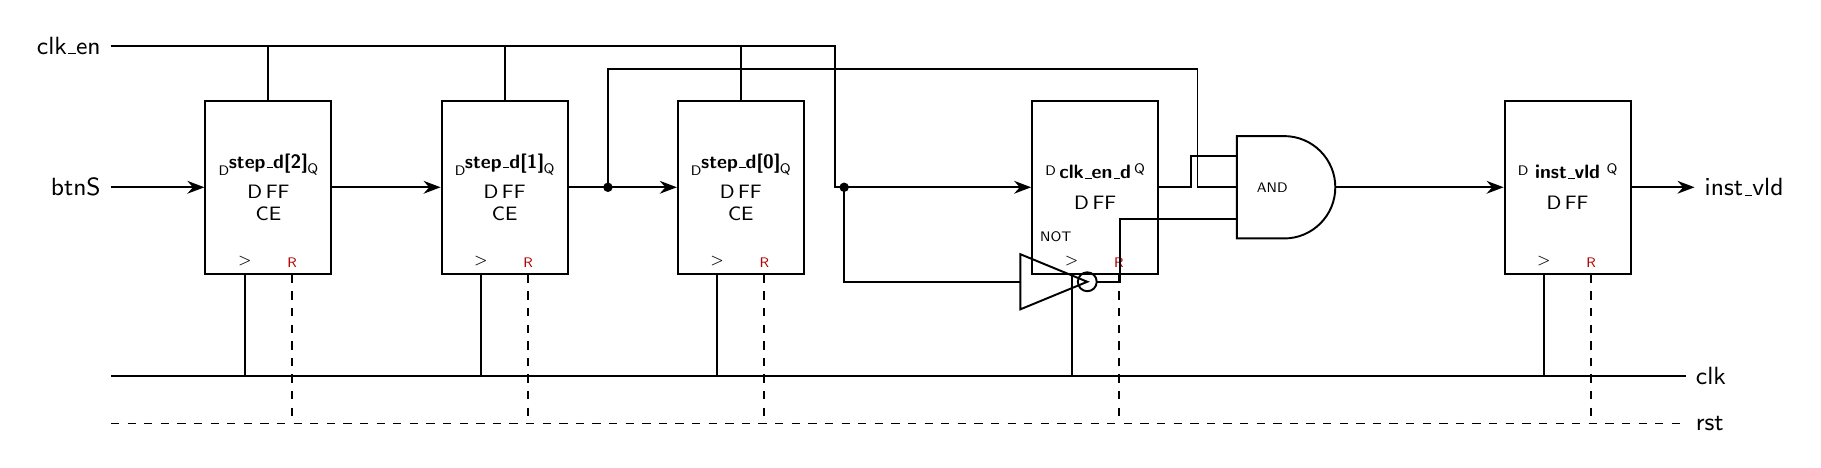
\begin{tikzpicture}[
        font=\sffamily\small,
        >=Stealth,
        line width=0.7pt,
        dff/.style={
            draw, rectangle,
            minimum width=1.6cm,
            minimum height=2.2cm,
            align=center,
            font=\sffamily\scriptsize
        },
    ]
    
    %============================================================
    % LAYOUT CONSTANTS
    %============================================================
    \def\sep{3.0}     % horizontal spacing between FF centres
    \def\yff{0}       % vertical centre of all FFs
    \def\clky{-2.4}   % clk bus y
    \def\rsty{-3.0}   % rst bus y
    \def\cey{1.8}     % clk_en bus y
    
    %============================================================
    % FLIP-FLOP NODES
    %============================================================
    \node[dff] (FF2)  at (0,        \yff) {{\bfseries step\_d[2]}\\[3pt]D\,FF\\CE};
    \node[dff] (FF1)  at (1*\sep,   \yff) {{\bfseries step\_d[1]}\\[3pt]D\,FF\\CE};
    \node[dff] (FF0)  at (2*\sep,   \yff) {{\bfseries step\_d[0]}\\[3pt]D\,FF\\CE};
    \node[dff] (FFCE) at (3.5*\sep, \yff) {{\bfseries clk\_en\_d}\\[3pt]D\,FF};
    \node[dff] (FFIV) at (5.5*\sep, \yff) {{\bfseries inst\_vld}\\[3pt]D\,FF};
    
    %============================================================
    % PORT COORDINATES
    %============================================================
    \foreach \ff in {FF2, FF1, FF0, FFCE, FFIV}{
        \coordinate (\ff-D)   at (\ff.west);
        \coordinate (\ff-Q)   at (\ff.east);
        \coordinate (\ff-CLK) at ($(\ff.south)+(-0.3,0)$);
        \coordinate (\ff-RST) at ($(\ff.south)+(0.3,0)$);
    }
    \foreach \ff in {FF2, FF1, FF0}{
        \coordinate (\ff-CE) at (\ff.north);
    }
    
    %============================================================
    % PORT LABELS (D, Q, >, R) inside each FF
    %============================================================
    \foreach \ff in {FF2, FF1, FF0, FFCE, FFIV}{
        \node[font=\sffamily\tiny, anchor=south west] at ($(\ff.west)+(0.05,0.02)$) {D};
        \node[font=\sffamily\tiny, anchor=south east] at ($(\ff.east)+(-0.05,0.02)$) {Q};
        \node[font=\sffamily\tiny] at ($(\ff.south)+(-0.3,0.18)$) {$\mathbf{>}$};
        \node[font=\sffamily\tiny, text=red!70!black] at ($(\ff.south)+(0.3,0.15)$) {R};
    }
    
    %============================================================
    % CLK BUS (solid horizontal line at bottom)
    %============================================================
    \draw (-2, \clky) -- (5.5*\sep+1.5, \clky) node[right] {clk};
    \foreach \ff in {FF2, FF1, FF0, FFCE, FFIV}{
        \draw (\ff-CLK) -- (\ff-CLK |- 0,\clky);
    }
    
    %============================================================
    % RST BUS (dashed horizontal line below clk)
    %============================================================
    \draw[dashed] (-2, \rsty) -- (5.5*\sep+1.5, \rsty) node[right] {rst};
    \foreach \ff in {FF2, FF1, FF0, FFCE, FFIV}{
        \draw[dashed] (\ff-RST) -- (\ff-RST |- 0,\rsty);
    }
    
    %============================================================
    % CLK_EN BUS (horizontal line above step_d FFs)
    %============================================================
    % clk_en enters from the left, runs above the three shift-register FFs
    \coordinate (ce_start) at (-2, \cey);
    \coordinate (ce_end)   at (2*\sep+0.8, \cey);
    \draw (ce_start) -- (ce_end);
    \node[left] at (ce_start) {clk\_en};
    
    % Branches down to CE ports of step_d[2], step_d[1], step_d[0]
    \foreach \ff in {FF2, FF1, FF0}{
        \draw (\ff-CE) -- (\ff-CE |- 0,\cey);
    }
    
    %============================================================
    % CLK_EN → D of clk_en_d
    % Route: from the ce bus end, go down and right to FFCE-D
    %============================================================
    \coordinate (ce_drop) at ($(ce_end)+(0.4,0)$);
    \draw[->] (ce_end) -- (ce_drop) -- (ce_drop |- FFCE-D) -- (FFCE-D);
    
    %============================================================
    % btnS → D of step_d[2]
    %============================================================
    \draw[->] (-2, \yff) node[left] {btnS} -- (FF2-D);
    
    %============================================================
    % SHIFT REGISTER CHAIN: FF2 Q → FF1 D → FF0 D
    %============================================================
    \draw[->] (FF2-Q) -- (FF1-D);
    \draw[->] (FF1-Q) -- (FF0-D);
    
    %============================================================
    % NOT GATE (inverter): input = step_d[0] Q
    % Placed below the main FF row, between FF0 and FFCE
    %============================================================
    \def\notx{10.0}   % x centre
    \def\noty{-1.2}   % y centre
    
    % Triangle body
    \draw (\notx-0.45, \noty+0.35)
       -- (\notx+0.4, \noty)
       -- (\notx-0.45, \noty-0.35) -- cycle;
    % Bubble
    \draw (\notx+0.4, \noty) circle[radius=0.12];
    \node[font=\sffamily\tiny, above] at (\notx, \noty+0.38) {NOT};
    
    \coordinate (NOTin)  at (\notx-0.45, \noty);
    \coordinate (NOTout) at (\notx+0.52, \noty);
    
    % Wire: FF0 Q → tap down → NOT input
    \coordinate (FF0tap) at ($(FF0-Q)+(0.5,0)$);
    \fill (FF0tap) circle[radius=0.06];  % junction dot
    \draw (FF0tap) -- (FF0tap |- 0,\noty) -- (NOTin);
    
    %============================================================
    % AND GATE (3-input): clk_en_d, step_d[1], NOT(step_d[0])
    % Placed to the right of the NOT gate
    %============================================================
    \def\andx{12.8}
    \def\andy{0}
    
    % AND gate body (flat left, curved right)
    \draw (\andx-0.5, \andy+0.65) -- (\andx-0.5, \andy-0.65)
       -- (\andx+0.1, \andy-0.65)
          arc[start angle=-90, end angle=90, radius=0.65]
       -- cycle;
    \node[font=\sffamily\tiny] at (\andx-0.05, \andy) {AND};
    
    \coordinate (ANDin1) at (\andx-0.5, \andy+0.4);   % top:  clk_en_d
    \coordinate (ANDin2) at (\andx-0.5, \andy);        % mid:  step_d[1]
    \coordinate (ANDin3) at (\andx-0.5, \andy-0.4);    % bot:  NOT(step_d[0])
    \coordinate (ANDout) at (\andx+0.75, \andy);
    
    % --- Wire: clk_en_d Q → AND top input ---
    \draw (FFCE-Q) -- ++(0.4,0) coordinate (CEtap)
       -- (CEtap |- ANDin1) -- (ANDin1);
    
    % --- Wire: step_d[1] Q → AND mid input (tap from chain) ---
    \coordinate (FF1tap) at ($(FF1-Q)+(0.5,0)$);
    \fill (FF1tap) circle[radius=0.06];  % junction dot
    \draw (FF1tap) -- (FF1tap |- 0,\andy+1.5)
       -- (\andx-1.0, \andy+1.5)
       -- (\andx-1.0, \andy) -- (ANDin2);
    
    % --- Wire: NOT output → AND bot input ---
    \draw (NOTout) -- ++(0.3,0) coordinate (NOTtap)
       -- (NOTtap |- ANDin3) -- (ANDin3);
    
    %============================================================
    % AND OUTPUT → D of inst_vld
    %============================================================
    \draw[->] (ANDout) -- ++(0.3,0) coordinate (ANDtap)
       -- (ANDtap |- FFIV-D) -- (FFIV-D);
    
    %============================================================
    % inst_vld OUTPUT
    %============================================================
    \draw[->] (FFIV-Q) -- ++(0.8,0) node[right] {inst\_vld};
    
    \end{tikzpicture}
    }
    \caption{Debounce shift register with rising-edge detector for \texttt{inst\_vld}}
    \end{figure}
    \end{enumerate}


\subsection{Register File}

The sequencer’s register file is located in a file called \texttt{seq\_rf.v}. It stores the values of the four registers. Take a look at the source code and see if you can understand how it is implemented. Answer the following questions in the lab report.



\textbf{Questions.}
\begin{enumerate}
    \item Find the line of code where a register is written a non-zero value. Is this sequential logic or combinational logic?

    \textit{Answer.} The line where the register is written a non-zero value is\\
    \begin{mdframed}
    \begin{minted}[fontsize=\footnotesize]{verilog}
rf[i_wsel] <= i_wdata;
    \end{minted}
    \end{mdframed}

    This is sequential logic, because it is inside an \verb|always @ (always @ (posedge clk))|, this means that the write only occurs on the rising edge of the clock. Also, the non-blocking assignment \verb|<=| is typical for flip-flop behavior. If they were using combinational, they'd be using the blocking assignment \verb|=|.
    
    \item Find the lines of code where the register values are read out from the register file. Is this sequential or combinational logic? If you were to manually implement the readout logic, what kind of logic elements would you use?

    \textit{Answer.} The lines of code where the register values are read out from the register files are:\\

    \begin{mdframed}
    \begin{minted}[fontsize=\footnotesize]{verilog}
assign o_data_a = rf[i_sel_a];
assign o_data_b = rf[i_sel_b];
    \end{minted}
    \end{mdframed}

    This is combinational logic, since we're using the blocking assignment, which is typical for combinational logic. Also, they use continuous assign statements — there is no clock involved. If we were to implement this manually, we would use a $4\times 2$ multiplexer.
    
    \item Draw a circuit diagram of the register file block. It should be a translation of the corresponding Verilog code.

\begin{figure}[H]
\centering
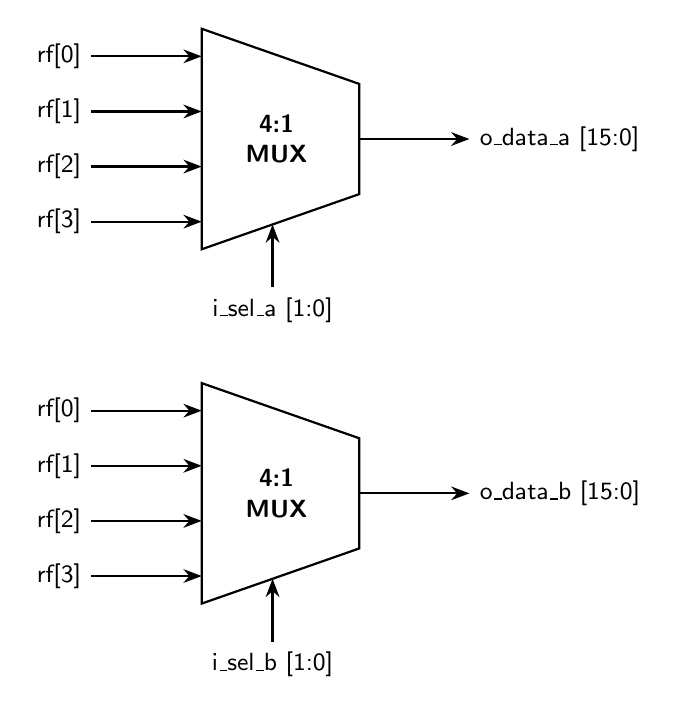
\begin{tikzpicture}[
    font=\sffamily\small,
    >=Stealth,
    line width=0.8pt,
]

%------------------------------------------------------------
% MUX geometry constants
%   wide face (left):  total height = 2*Hw
%   narrow face (right): total height = 2*Hn
%   depth (left to right): D
%------------------------------------------------------------
\def\D{2.0}    % depth
\def\Hw{1.4}   % half-height, wide face
\def\Hn{0.7}   % half-height, narrow face

%============================================================
%  MUX A
%============================================================
% Wide-face centre at origin
\coordinate (AW) at (0,0);
\coordinate (AN) at (\D,0);

% Four corners
\coordinate (AWt) at (0, \Hw);
\coordinate (AWb) at (0,-\Hw);
\coordinate (ANt) at (\D, \Hn);
\coordinate (ANb) at (\D,-\Hn);

% Trapezoid body
\draw (AWt) -- (ANt) -- (ANb) -- (AWb) -- cycle;

% Label
\node[font=\sffamily\bfseries\small, align=center] at (0.95,0) {4:1\\MUX};

% --- 4 data inputs, evenly spaced on the wide face ---
% positions: top-quarter, upper-mid, lower-mid, bottom-quarter
\foreach \i/\lbl in {0/rf{[0]}, 1/rf{[1]}, 2/rf{[2]}, 3/rf{[3]}}{
    % y goes from +3Hw/4 down to -3Hw/4 in steps of Hw/2
    \pgfmathsetmacro\yy{\Hw - (2*\Hw/4)*(\i + 0.5)}
    \coordinate (Ain\i) at (0, \yy);
    \draw[->] (-1.4, \yy) -- (0, \yy);
    \node[left] at (-1.4, \yy) {\lbl};
}

% --- Select input: vertical arrow entering bottom of body ---
\pgfmathsetmacro\selx{\D*0.45}   % x position along body where sel enters
% Intersection of a vertical line x=selx with the bottom edge AWb->ANb
% Bottom edge goes from (0,-Hw) to (D,-Hn): parametric y = -Hw + (Hw-Hn)*t, x = D*t
% At x=selx: t = selx/D, so y = -Hw + (Hw-Hn)*(selx/D)
\pgfmathsetmacro\sely{-\Hw + (\Hw-\Hn)*(\selx/\D)}
\draw[->] (\selx, \sely-0.8) -- (\selx, \sely);
\node[below, font=\sffamily\small] at (\selx, \sely-0.8) {i\_sel\_a [1:0]};

% --- Output on narrow face ---
\coordinate (Aout) at (\D, 0);
\draw[->] (\D, 0) -- (\D+1.4, 0);
\node[right] at (\D+1.4, 0) {o\_data\_a [15:0]};


%============================================================
%  MUX B  (offset downward)
%============================================================
\def\Yb{-4.5}

\coordinate (BWt) at (0, \Yb+\Hw);
\coordinate (BWb) at (0, \Yb-\Hw);
\coordinate (BNt) at (\D, \Yb+\Hn);
\coordinate (BNb) at (\D, \Yb-\Hn);

\draw (BWt) -- (BNt) -- (BNb) -- (BWb) -- cycle;

\node[font=\sffamily\bfseries\small, align=center] at (0.95, \Yb) {4:1\\MUX};

\foreach \i/\lbl in {0/rf{[0]}, 1/rf{[1]}, 2/rf{[2]}, 3/rf{[3]}}{
    \pgfmathsetmacro\yy{\Yb + \Hw - (2*\Hw/4)*(\i + 0.5)}
    \draw[->] (-1.4, \yy) -- (0, \yy);
    \node[left] at (-1.4, \yy) {\lbl};
}

\pgfmathsetmacro\sely{\Yb - \Hw + (\Hw-\Hn)*(\selx/\D)}
\draw[->] (\selx, \sely-0.8) -- (\selx, \sely);
\node[below, font=\sffamily\small] at (\selx, \sely-0.8) {i\_sel\_b [1:0]};

\draw[->] (\D, \Yb) -- (\D+1.4, \Yb);
\node[right] at (\D+1.4, \Yb) {o\_data\_b [15:0]};

\end{tikzpicture}
\caption{Register File — Read Port Multiplexers}
\end{figure}

\item Capture a waveform that shows the first time register 3 is written with a 
non-zero value.

\begin{figure}[H]
    \centering
    \begin{tikzpicture}
        \node[anchor=south west, inner sep=0] (img) at (0,0) {
            \includegraphics[width=0.8\linewidth]{image3.png}
        };
        \begin{scope}[x={(img.south east)},y={(img.north west)}]
            % Circles
            \draw[red, thick]  (0.59, 0.12) circle [radius=0.03];
            \draw[blue, thick] (0.67, 0.06) circle [radius=0.03];

            % Arrow to red circle (from below image)
            \draw[->, red, thick] (0.52, -0.12) -- (0.59, 0.12);
            \node[red, below, font=\sffamily\small] at (0.52, -0.12) {register 2};

            % Arrow to blue circle (from below image)
            \draw[->, blue, thick] (0.74, -0.18) -- (0.67, 0.06);
            \node[blue, below, font=\sffamily\small] at (0.74, -0.18) {register 3};
        \end{scope}
    \end{tikzpicture}
    \caption{Captured waveform with \texttt{rf[2][15:0]} and \texttt{rf[3][15:0]}}
\end{figure}


\end{enumerate}



\section{Workshop 2}

\subsection{Nicer UART Output}

The existing testbench program contains a UART model that announces each byte that’s received by the model. While generic, the output of this model is somewhat hard to read. Modify \texttt{model\_uart.v} such that the per-byte output is suppressed. Instead, \texttt{model\_uart.v} shall output one line at a time after a carriage-return character (\texttt{\textbackslash r}) is received. For example, print out \texttt{``0003\textbackslash n''} instead of \texttt{``0\textbackslash n'' ``0\textbackslash n'' ``0\textbackslash n'' ``3\textbackslash n''} for the first line of UART output.

\textbf{Note:} you are only allowed to use \texttt{\$display} in this task (e.g. no \texttt{\$write} is allowed). We suggest that you read the UART protocol to further understand the test bench before starting to work on the task.

\textit{Answer.} We first add the two lines for the buffer\\

\begin{mdframed}
\begin{minted}[fontsize=\footnotesize]{verilog}
output TX;
input  RX;

// add these new two lines
reg [8*32-1:0] line_buf;  // up to 32 characters
integer        idx;
\end{minted}
\end{mdframed}

We then modify the following part below:\\

\begin{mdframed}
\begin{minted}[fontsize=\footnotesize]{verilog}
   always @ (negedge RX)
     begin
        rxData[7:0] = 8'h0;
        #(0.5*bittime);
        repeat (8)
          begin
             #bittime ->evBit;
             //rxData[7:0] = {rxData[6:0],RX};
             rxData[7:0] = {RX,rxData[7:1]};
          end
        ->evByte;
        $display ("%d %s Received byte %02x (%s)", $stime, name, rxData, rxData); // modify this
     end
\end{minted}
\end{mdframed}

Into this:\\

\begin{mdframed}
\begin{minted}[fontsize=\footnotesize]{verilog}
   always @ (negedge RX)
     begin
        rxData[7:0] = 8'h0;
        #(0.5*bittime);
        repeat (8)
          begin
             #bittime ->evBit;
             //rxData[7:0] = {rxData[6:0],RX};
             rxData[7:0] = {RX,rxData[7:1]};
          end
        ->evByte;

        // modified code
        if (rxData == 8'h72) begin  // 'r'
            line_buf[8*idx +: 8] = 8'h00; // null terminate
            $display("%s", line_buf);
            line_buf = 0;
            idx = 0;
        end
        else if (rxData != 8'h0A) begin  // ignore '\n'
            line_buf[32 - 8 - 8*idx +: 8] = rxData;
            idx = idx + 1;
        end
     end
\end{minted}
\end{mdframed}

\subsection{An Easier Way to Load Sequencer Program}

The existing sequencer testbench sends a static sequence of instructions to the UUT (Unit Under Test) after the reset. In the last session you have observed this in the waveform viewer how the instructions are sent. Answer the following questions in your lab report.

\textbf{Questions.}

\begin{enumerate}
    \item Identify the part of the \texttt{tb.v} where the instructions are sent to the UUT.

    \textit{Answer.} The part of the \texttt{tb.v} where the instructions are sent to the UUT is:\\
    
    \begin{mdframed}
    \begin{minted}[fontsize=\footnotesize, linenos]{verilog}
task tskRunInst;
   input [7:0] inst;
   begin
      $display ("%d ... Running instruction %08b", $stime, inst);
      sw = inst;                 // instruction applied here
      #1500000 btnS = 1;         // trigger execution
      #3000000 btnS = 0;
   end
endtask
    \end{minted}
    \end{mdframed}
    However, the loop that feeds instructions is in the initial block:\\

    \begin{mdframed}
    \begin{minted}[fontsize=\footnotesize, linenos]{verilog}
for(idx = 1; idx <= instr_count; idx = idx + 1) begin
    tskRunInst(instr_mem[idx]);   // instructions sent here
end
    \end{minted}
    \end{mdframed}
    
    \item Which user tasks are called in this process?

    \textit{Answer.} Only one task is actually called directly, which is \verb|tskRunInst|. However, there are additional helper tasks defined:\\
    
    \begin{mdframed}
    \begin{minted}[fontsize=\footnotesize]{verilog}
tskRunPUSH
tskRunSEND
tskRunADD
tskRunMULT
    \end{minted}
    \end{mdframed}

    These tasks construct instruction encodings, then they internally call \verb|tskRunInst|. However, note that they are not used in the main loop
\end{enumerate}

Now we would like to change the static set of instructions. Instead, we will be loading instructions from a text file. The format of the file is the following:

\begin{enumerate}
    \item The name of the file is \texttt{``seq.code''}
    \item The file is up to 1024 lines long.
    \item The first line of the file contains a binary number that indicates how many instructions are included in this file.
    \item Each of the remaining $(n-1)$ lines contains a single instruction in binary.
\end{enumerate}

For example, here’s the file-equivalent of the simple sequencer instructions currently in use:\\

\begin{mdframed}
\begin{minted}[fontsize=\footnotesize, linenos]{text}
1010
00000100
00000000
00010011
10000110
01100011
10011111
11000000
11010000
11100000
11110000
\end{minted}
\end{mdframed}



\textbf{Modify the testbench such that it loads \texttt{seq.code} into an array, and executes every instruction in the file.}

\textbf{Hint:} for file I/O, you may use the built-in Verilog system task \texttt{\$readmemb} (google Verilog quick reference), or the C-like \texttt{\$fopen} and \texttt{\$fscanf} tasks.

\textbf{Hint:} Add \texttt{seq.code} in from add sources $\rightarrow$ Add or create simulation sources. (to see the file you should scroll down to All Files in)

\textit{Answer.} We modify \verb|tb.v| by first adding the following:
\begin{itemize}
    \item A memory array of 1024 entries, each 8 bits wide (a byte-addressable instruction memory)
    \item A 32-bit signed integer used to track how many instructions were loaded
\end{itemize}

Translating this into code, we have:\\

\begin{mdframed}
\begin{minted}[fontsize=\footnotesize]{verilog}
reg [7:0] instr_mem [0:1023];  // up to 1024 instructions
integer instr_count;
integer idx;    // used for later in the loop, declare in module level
\end{minted}
\end{mdframed}


Then, simply load the content from the file into the array:\\

\begin{mdframed}
\begin{minted}[fontsize=\footnotesize]{verilog}
// modify path here
// I used absolute path so I can put it in my desired folder
$readmemb("/home/don-le/Documents/FPGA/Verilog/lab_1/input/seq.code", instr_mem);
instr_count = instr_mem[0];
\end{minted}
\end{mdframed}

Finally, we execute the instruction from the file using \verb|tskRunInst|:\\

\begin{mdframed}
\begin{minted}[fontsize=\footnotesize]{verilog}
for(idx = 1; idx <= instr_count; idx = idx + 1) 
begin
    tskRunInst(instr_mem[idx]);
end
\end{minted}
\end{mdframed}

\subsection{Fibonacci Numbers}

Now that you have an easier way to program the sequencer from simulation, design a sequence of instructions such that the first 10 numbers of the Fibonacci series is printed from the UART.

\textit{Answer.}\\

\begin{mdframed}
\begin{minted}[fontsize=\footnotesize, linenos]{text}
101000
00000000
00010001
00110000
11000000
01000110
01011100
01101101
11000000
01000110
01011100
01101101
11000000
01000110
01011100
01101101
11000000
01000110
01011100
01101101
11000000
01000110
01011100
01101101
11000000
01000110
01011100
01101101
11000000
01000110
01011100
01101101
11000000
01000110
01011100
01101101
11000000
01000110
01011100
01101101
11000000
\end{minted}
\end{mdframed}


\section{Conclusion}

In this lab we explored the architecture of a simple 8-bit sequencer implemented on the Basys-3 FPGA board. We studied the clock divider that derives a ${\sim}763$\,Hz enable signal from the 100\,MHz master clock, the debounce shift-register that produces a clean single-cycle \texttt{inst\_vld} pulse, and the 4-register register file with combinational read ports and a synchronous write port. On the testbench side, we modified the UART model to buffer characters and print one line at a time, replaced the hard-coded instruction sequence with file-based loading via \texttt{\$readmemb}, and verified correctness by programming the sequencer to output the first ten Fibonacci numbers.

\end{document}